% !Mode:: "TeX:UTF-8"
%!TEX program  = xelatex

\documentclass[withoutpreface,bwprint]{cumcmthesis}


\coursename{ACM-ICPC 算法与程序设计}
\title{基于不相交集的问题求解报告}
\schoolname{微电子与固体电子学院}
\studentid{2016030102010}
\xuankehao{}
\author{傅宣登}
\theteacher{杨鹏}

\begin{document}
\maketitle
\begin{abstract}

不相交集是一种常用的数据结构。这种数据结构实现简单,操作迅速。

简单地说,不相交集可用于快速查询一堆元素是否属于同一集合。
鉴于在有些问题中,这种关系相当隐秘,本文采用另一种更理论的方式来描述这种关系。

本文讨论了实现不相交集的基础数据结构:数组、红黑树、树。本文采用树来实现不相交集。
接着给出了朴素的求并、查询算法,然后用所谓的路径压缩优化了查询算法。

最后给出了一道例题,并写出了完整的求解报告。

\keywords{不相交集\quad  算法\quad   数据结构\quad  程序设计}
\end{abstract}

\begin{center}%
	{\zihao{4}\heiti 正文 \vspace{-.5em}}%
\end{center}%

\section{不相交集 ADT}

不相交集(并查集)是描述解决等价问题的一种有效数据结构。
这种数据结构实现起来非常简单,而且每种操作只需要常数平均时间。
许多算法中都用到了不相交集,例如 \verb|Kruskal| 算法和 \verb|Prim| 算法等。

\subsection{等价关系}

若对每一对元素 $(a, b),\ \ a,b \in S$,$aRb$ 要么为 \verb|true| 要么为 \verb|false|,
则称在集合 $S$ 上定义关系 $R$。
如果 $aRb$ 是 \verb|true|,那么我们说 $a$ 与 $b$ 有关系。

\begin{definition}[等价关系]
等价关系是满足下列三个性质的关系 $R$:
\begin{itemize}
\item (自反性)对于所有的 $a\in S$,$aRa$;
\item (对称性)$aRb$ 当且仅当 $bRa$;
\item (传递性)若 $aRb$ 且 $bRc$,则 $aRc$。
\end{itemize}
\end{definition}

这里有几个例子。

如果两个城市位于同一个国家,那么定义他们是有关系的。容易验证这是一个等价关系。
如果能够通过公路从城镇 $a$ 旅行到 $b$,则设 $a$ 与 $b$ 有关系。
如果所有的道路都是双向行驶的,那么这种关系也是一个等价关系。

\subsection{动态等价性问题}

给定一个等价关系“$\sim$”,一个自然的问题是对任意的 $a$ 和 $b$,确定是否 $a\sim{}b$。
如果将等价关系存储为一个二维布尔数组,那么当然这个工作可以以常数时间完成。
问题在于这种关系的定义通常不明显甚至相当隐秘。

例如,设在5个元素的集合 $\{a_1,a_2,a_3,a_4,a_5\}$ 上定义一个等价关系。
此时存在25对元素,他们的每一对要么有关系要么没有关系。
然而,信息 $a_1\sim{}a_2, a_3\sim{}a_4, a_4\sim{}a_2, a_1\sim{}a_5$ 意味着每一对元素都是有关系的。
我们需要一个能快速判断出这些关系的数据结构。

\begin{definition}[等价类]
一个元素 $a\in{}S$ 的等价类是 $s$ 的一个子集,它包含所有与 $a$ 有关系的元素。
\end{definition}

显然,等价类形成对 $S$ 的一个划分:$S$ 的每一个元素恰好出现在一个等价类中。
这样,为确认是否 $a\sim{}b$,我们只需验证 $a$ 和 $b$ 是否都在同一个等价类中。

输入数据最初是由 $N$ 个集合的类,每个集合含有一个元素。
初始的描述是所有的关系均为假(自反的关系除外)。
每个集合都有一个不同的元素,从而 $S_i\cap{}S_j = \varPhi$;
即所有集合不相交。

此时,我们定义两种运算。
第一种是 \verb|Find|,它返回包含给定元素的集合(即等价类)的名字。
第二种是添加关系。
如果我们想要添加关系 $a\sim{}b$,那么我们首先要看是否 $a$ 和 $b$ 已经有关系。
这可以通过对 $a$ 和 $b$ 执行 \verb|Find| 并检查它们是否在同一个等价类中来完成。
如果它们不在同一个等价类中,那么我们使用求并运算 \verb|Union|,这种运算把含有 $a$ 和 $b$ 的两个等价类合并成一个新的等价类。
从集合的观点看,$\cup$ 的结果是建立一个新集合 $S_k = S_i \cup S_j$,并去掉原来两个集合而保持所有的集合的不相交性。
由于这个原因,常常把这项工作的算法叫做不相交集的 \verb|Union|/\verb|Find| 算法,不相交集也叫并查集。

很容易观察到,该算法是动态的。因为在算法执行的过程中,集合可以通过 \verb|Union| 运算而发生变化。
另外,由 \verb|Find| 返回的集合的名字实际上是相当任意的。
真正重要的关键在于:当 $a$ 和 $b$ 在同一个集合中的时候,$\mathrm{Find}(a) = \mathrm{Find}(b)$。

解决动态等价性问题的方案有两种。
一种方案保证指令 \verb|Find| 能够以常数最坏情形运行时间执行,
而另一种方案则保证指令 \verb|Union| 能够以常数最坏情形运行时间执行。
曾有人指出二者不能同时做到。

\section{不相交集的实现}

本文将考查 \verb|Union|/\verb|Find| 问题的一种解法,
其中每次操作的执行时间几乎是常数时间。

\subsection{基本数据结构}

%\subsubsection{容器的选择}
注意到动态等价性问题并不要求 \verb|Find| 操作返回任何特定的名字,
而只是要求当且仅当两个元素属于同一个集合时,
作用在这两个元素上的 \verb|Find| 返回相同的名字。

于是有多种容器可以用来实现并查算法,例如树、数组(向量)、集合(红黑树)等,
本文仅讨论使用树来表示集合的实现方法。
由于树上每一个元素都有相同的根,
这样该根就可以用来命名所在的集合。

虽然这些树不一定是二叉树,但要表示他们却相当的容易,因为需要存储的唯一信息就是一个父指针。
集合的名字由根节点给出。
可以用一个数组存储这些树,数组中每个成员 $P[i]$ 表示元素 $i$ 的父节点。
如果 $i$ 是根,那么 $P[i] = i$。

初始时,对于 $1\le i \le N,\,{}P[i] = i$。

\subsection{并查算法}

对元素 $X$ 执行 $\mathrm{Find}(X)$ 操作会返回包含 $X$ 的的树的根,
这可以通过不断对它的父节点执行 \verb|Find| 操作完成。
\begin{lstlisting}{language=C}
Find(x):
	if P[x] == x
		return x;
	else
		return Find(P[x]);
\end{lstlisting}
执行这次操作的时间与表示 $X$ 的节点的深度成正比。

为了执行两个元素的 \verb|Union| 运算,只需使一个节点的根指向另一棵树的根节点。
\begin{lstlisting}{language=C}
Union(x, y):
	P[ Find(x) ] = P[ Find(y) ];
\end{lstlisting}

上面伪代码表示的基本算法的实现中,假设差错检验已经执行。

\subsection{路径压缩}

如果存在大量对深节点的 \verb|Find| 操作,
那么将重复执行很多次相同的递归调用,这是非常浪费时间的。
于是可以考虑每次执行 \verb|Find| 操作时,
将该节点的根节点修改为其树的根节点,以减少将来访问的时间。

\begin{lstlisting}{language=C}
Find(x):
	if P[x] == x
		return x;
	else
		return P[x] = Find(P[x]);
\end{lstlisting}

优化后的算法在最坏情形下几乎是线性的。在最坏情况下需要的时间是
$\Theta(M\alpha(M,N))$ (假设 $M\ge N$),
其中 $\alpha(M, N)$ 是 Ackermann 函数的逆。

\section{例题:TROY Query}

以 Codeforces Hello 2015 (Div. 2) 的 F 题\footnote{http://codeforces.com/gym/100571/problem/F}。

\section{符号说明}

\begin{tabular}{cc}
 \hline
 \makebox[0.4\textwidth][c]{符号}	&  \makebox[0.5\textwidth][c]{意义} \\ \hline
 D	    & 木条宽度(cm) \\ \hline
 L	    & 木板长度(cm)  \\ \hline
 W	    & 木板宽度(cm)  \\ \hline
 N	    & 第n根木条  \\ \hline
 T	    & 木条根数  \\ \hline
 H	    & 桌子高度(cm)  \\ \hline
 R	    & 桌子半径(cm)  \\ \hline
 R	    & 桌子直径(cm)  \\ \hline
\end{tabular}

\section{问题分析}

\subsection{问题三分析}
题目要求制作软件的意思就是客户给定折叠桌高度、桌面边缘线的形状大小和桌脚边缘线的大致形状,将这些信息输入程序就得到客户想要的桌子。我们在求解最优设计加工参数时,自行给定桌面边缘线形状(椭圆、相交圆等),桌脚边缘线形状,折叠桌高度,应用第二问的非线性规划模型,用MATLAB软件绘制折叠桌截面图,得到自己设计的创意平板折叠桌。

问题三流程图:
%\begin{figure}[!h]
%\centering
%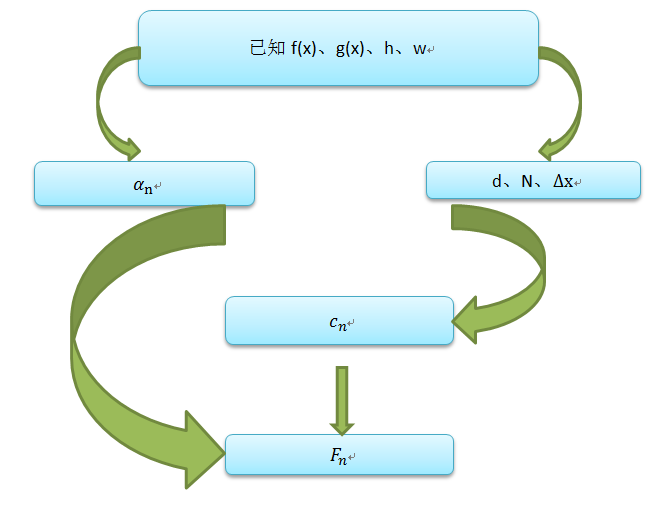
\includegraphics[width=\textwidth]{1.png}
%\caption{问题三流程图}
%\end{figure}

%参考文献
\bibliographystyle{unsrt}
\nocite{*}
\bibliography{reference}

\newpage
%附录
\appendix
\section{Hello 源代码}
\lstinputlisting[language=C]{src/hello.c}


\end{document} 